\documentclass[UTF8]{ctexart}
\usepackage{shumo}%可以点开查看宏包和定义内容,同时可以自行另外加宏包和定义
\geometry{left=2.50cm,right=2.5cm,top=2.50cm,bottom=2.5cm}%页面布局集训标准,可自行适当修改
%====================================================
%设置附录代码的格式,可以自行修改
\lstset{
	breaklines=true,% 允许自动断行
	% breakatwhitespace=true,% 使用此命令仅允许在空格处自动断行
	showstringspaces=false,% 不显示字符串中的空格
	basicstyle=\small\ttfamily,% 设置代码基本样式
	flexiblecolumns=true,% 改善字母间距
	keywordstyle=\color{blue},% 设置关键词样式
	stringstyle=\color[rgb]{0.75,0,0.75},% 设置字符串样式
	commentstyle=\songti\color[rgb]{0,0.5,0},% 设置注释样式
	tabsize=4,% 设置制表符缩进
}
%====================================================
\title{\textbf{基于逻辑斯蒂模型的网络信息传播研究}}% 请勿修改
\date{}%请勿添加自己的信息
\author{}%请勿添加自己的信息
%下面时正文
\begin{document}
\setcounter{page}{1}%从正文开始计算页码	
\maketitle
\vspace{-0.95cm}
\thispagestyle{fancy}   
\fancyhf{} %清除原本页眉页脚形式
\renewcommand{\headrulewidth}{0pt} %页眉线宽,设为0可以去页眉线
%=================================================
%=================================================
%=================================================
%=================================================
%=================================================
%=================================================
%下面开始出现各位需要修改的部分。
	\renewcommand{\abstractname}{\sihao 摘\quad 要} %更改摘要二字的样式
\begin{abstract}\xiaosihao
	\vspace{0.1cm}
	\begin{spacing}{1.4}\xiaosihao
	在当今互联网基础设施高度发达的背景下,信息流传播范围和速度比以往任何时候都更为广泛和迅速。由于预测信息流则能够帮助我们在未来的信息传播中做出更为准确和优化的决策,从而更好地应对变化和挑战。因此本文根据已有数据建立网络信息传播模型,以便了解信息传播的机理并加以控制。\par
	针对问题一,\textbf{本文利用文件中信息传播的原始数据,结合生物学、传播学知识建立信息流转量模型。}考虑到媒体传播以及接收者的实际情况,本文选取取逻辑斯蒂模型。因此分析信息流转量模型时,可以从自由增长模型开始分析,引进逻辑斯蒂阻滞增长模型,构成信息流转初步框架。再者原始数据基于逻辑斯蒂模型进行非线性拟合,\textbf{可以得到信息的传播模型为$x\left( t \right) =\frac{664.0086}{1+72.7787\times \exp \left( -0.5491t \right)}$。}\par
	针对问题二,本文基于问题一的模型建立,队问题一中的公式进行微分分析,\textbf{得到信息传播速率的极值点是x=/$x_m$/2},并对问题一的模型进行变形计算得到在理论分析下的最快传播时间节点。之后本文利用了步长逼近的方法,在确定了目标的时间节点后,\textbf{对其进行遍历校验},最后得到最快传播时间节点计算正确,\textbf{在时间为t=7.81h时达到最大的传播速率为91.15。}\par
	针对问题三,本文通过已有的信息流转量模型来描述网络信息的传播情况,同时根据模型对于未来情况进行一定程度上的推广,在信息传播数据充分时利用数值微分和线性拟合化技术来估算相关参数,可以更加有效预测未来的信息传播速度,\textbf{将t=28带入公式可以得到28h时的信息流转量为663.998438。}\par
	针对问题四,本文根据0h~20h小时的信息流转量数据,运用数值微分得到年增长率的值,然后利用MATLAB软件线性拟合为如下直线方程r=c+d,\textbf{估算得到最大的的信息流转量$x_m=664.0086$}。\par
	针对问题五,在本文的假设中,\textbf{信息传播速度最快是在信息流转量量达到最大流转量一半的时候},因此可以知道,如果想要达到最快速的传播效果,使得流转量保持在最大流转量的一半是个最好的办法。同理,为了控制传播速度,需要尽可能在传播开始时加以限制。\par
	%这里填写你自己的关键词
	\end{spacing}
	\\ \hspace*{\fill} \\
	\textbf{关键词}:\quad 逻辑斯蒂模型,环境容纳量,传播因子分析,微分方程,回归拟合
\end{abstract}

\newpage

\pagestyle{plain}
%标准 LaTeX 提供下列四种页版式,可用 \pagestyle{页版式} 命令来设置页面版式:
%empty(没有页眉和页脚),plain(本次用的,无页眉,页脚为居中页码),headings(页眉为章节标题,无页脚),myheadings(页眉内容可自定义,无页脚)


\section{问题背景}
\subsection{问题背景}
当代网络信息传播背景的主要特点是高度互联和便利性。随着互联网技术的不断发展和完善,我们现在可以通过各种网络渠道获取到任何我们想要的信息。一个人只需要通过智能手机、电脑或平板电脑等设备连接网络,就可以获取各种官方和非官方信息,包括国内外新闻、娱乐、体育、科技等方面的资讯。同时,多种社交媒体和分享平台让任何人都可以轻松分享自己的观点和内容到全球范围内,从而让信息流无所不在。\par
现在,只需几秒钟的时间,就能把重要的新闻分享给全世界,这为我们带来无限便利和机遇。同时,网络媒体的崛起也使新闻传播变得更加平民化,人们可以直接通过互联网获取新闻信息并分享给自己的朋友和社交圈。这也让传播信息变得更加容易和普及,但同时也正是因为如此,我们需要更加深入地了解信息传播的机理、控制和预测以保证信息传播的准确、合法和可靠,这对于我们的个人和社会发展都至关重要。控制能够有利于我们更好地利用信息流传播和管理方式,掌握更多的信息资源,更好地了解世界和社会发展动态,同时也能更好地规划个人和企业的发展方向。\par 

\subsection{问题重述}
根据题目背景及所给附件,我们需要解决以下问题:\par
1.通过已知的时间——信息流转量数据,建立合适的网络信息传播模型。\par
2.根据已有数据,找出网络信息传播速度最快的时间点。\par
3.根据已有数据,预测在28h时信息的流转量。\par
4.通过模型分析最终的信息流转量能达到多少。\par 
5.对于信息传播过程中,提供一些控制传播速度的方式,并说明提供方式的有效性。\par 

\section{问题分析}
\subsection{问题背景的分析}
信息流的传播机理可以概括为信息源、传播媒介和接收者三个关键要素之间的互动过程。具体来说,每个信息流的传播过程中,都存在着以下三个基本要素:\par
信息源:信息源是信息流的起点,是信息的产生者或发起者。\par
传播媒介:传播媒介指将信息源传递给接收者的工具或渠道。它可以是电视、收音机、报纸、杂志、互联网等等,其中每种传播媒介都有其独特的特征和优势。\par
接收者:接收者是信息流的最终目的地,信息流的最终受众。接收者接受信息的方式和响应方式都是影响信息流传播的重要因素。\par
值得注意的是,信息源、传播媒介和接收者之间的相互作用是一个互动过程,因此,信息流的传播通常是循环和渐进的。在整个传播过程中,每个要素都会相互影响和影响过程的发展方向与传递效果。\par
\subsection{问题一的分析}
当仅考虑信息的传播时,信息在传播途径良好且无外力干扰的情况下,其传播数量应该是呈现指数型增长的,但是接收者会根据他们对信息的态度、信仰、背景和价值观调整他们的反应。同时,假设接收者之间存在相互影响的社交网络。因此本文采用描述种群生态的逻辑斯蒂模型来模拟信息的传播。\par
\subsection{问题二的分析}
利用逻辑斯蒂模型可以表征种群的数量动态,在实际的情况中,信息的传播速率受到例如网络资源的限制等多种因素的影响,最后在网络信息传播趋近于饱和时候,网络信息的传播速度会接近于0,因此可以通过微分的方法计算得到每一个时刻网络信息的传播速率并寻找其中的最大值。\par
\subsection{问题三的分析}
可以通过已有的模型来描述网络信息的传播情况,同时根据模型对于未来情况进行一定程度上的推广,可以通过预测分析得到28h时的信息流转量。\par
\subsection{问题四的分析}
在利用逻辑斯蒂模型描述种群数量问题时,有一个变量$x_m$来描述在某个环境中的最大群众数量接纳能力。同样地,考虑到有限的人数以及网络接受能力,网络信息的传播会在趋近最大值时传播速率接近于0,因此可以通过分析模型来得到可能的最大信息流转量。\par
\subsection{问题五的分析}
通过微分建模得到网络信息传播速率的模型公式,可以得到网络信息传播速率与信息源、传播媒介和接收者之间的关系,同时考虑实际的社会情况,可以给出实际的方式。例如加入对传播媒介的考虑,可以加入传播媒介限制:传播媒介的限制对信息传输速度也有着重要的影响。限制信息的传播媒介可能包括禁止某些媒介的使用或向接收者暂缓信息的提供。\par
\section{假设与符号说明}
\subsection{基本假设}
1.假设在网络信息传播中,仅考虑固定区域内的传播情况,忽略外界的影响因素。\par 
2.假设网络信息的传播仅和信息源、传播媒介和接收者有关。\par 
3.假设在传播开始后,仅考虑内部传播,不考虑更多的信息源。\par 
4.假设在信息传播中没有接收者人数的变化。\par 
5.假设接收者之间存在社交和影响网络。\par 
6.假设信息在传播过程中不会被改变。\par 
\subsection{符号说明}
\begin{table}[htbp]
	\centering 
	\begin{tabular}{lcr}
		\toprule
		变量名 & 符号说明 & 单位 \\
		\midrule
		$t$ & 时间& h \\
		${x_m}$ & 最大的的信息流转量 & $-$ \\
		$r$ & 网络信息的传播速度 & $-$ \\
		$x$ & 网络信息传播量 & $-$ \\
		\bottomrule
	\end{tabular}
\end{table}
\section{模型的建立与求解}
\subsection{问题一的模型建立}
根据题目中所给的数据,可以绘制出信息流转量随时间的变化关系,得到如下图一。\par 
\begin{figure}[h]
	\centering
	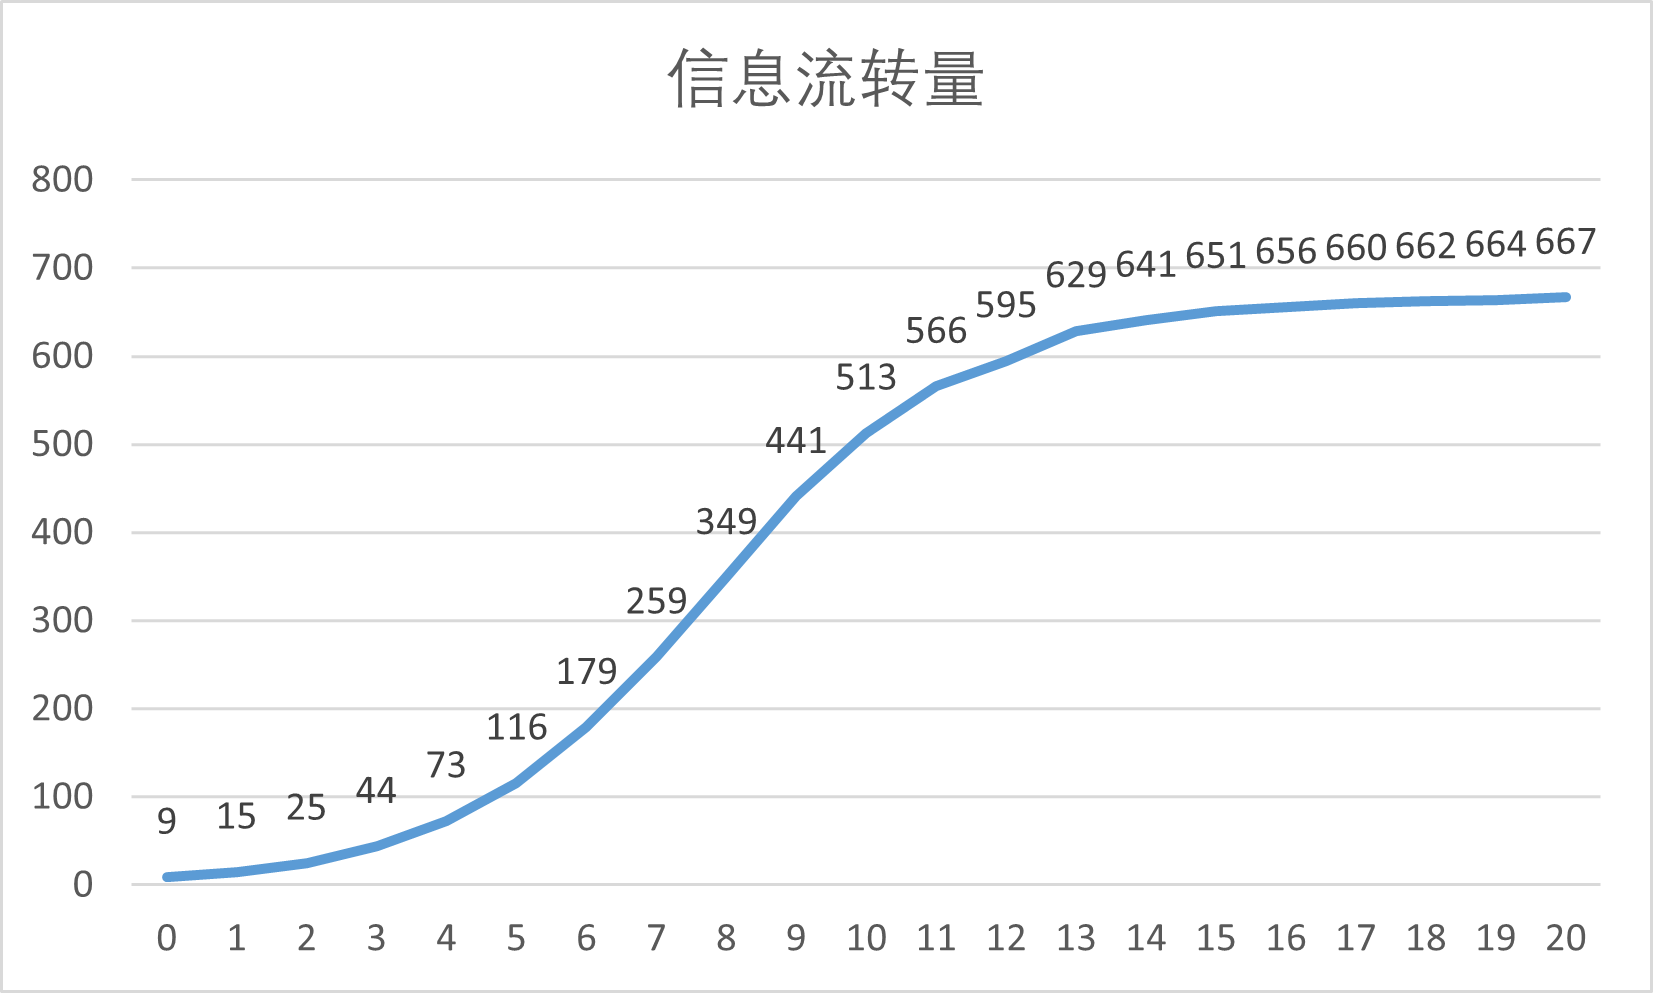
\includegraphics[scale=1]{信息流转量.png}
	\caption{信息流转量}
\end{figure}\par 
可以发现信息流转量随时间的变化大致呈显S型增长的趋势。考虑到信息流转对网络资源的竞争,可以假设信息传播速率r是信息流转量x(t)的函数r(x),即不同密度的信息量有不同的传播速率。逻辑斯蒂模型假设r(x)是x(t)的减函数且是x的线性函数r(x)=r-sx,s>0,这里的r相当于x(t=0)时的增长率r(x)<r,即网络传播媒介没有资源限制时的固有传播速率。显然实际传播速率为了明确参数s的实际意义,引入最大的信息流转量$x_m$,即目前网络信息媒介所能容纳的最大信息流转量。则当x=xm时,信息的传播速率为零,即0=r-s$x_m$;s=r/$x_m$,在逻辑斯蒂模型的线性假设下,有以下的模型\par
\begin{equation}
\frac{\mathrm{d}x}{\mathrm{d}t}=r\left( 1-\frac{x}{x_m} \right) 
\end{equation}\par
用分析变量法求解微分方程(1)可以得到上式的解为\par
\begin{equation}
x\left( t \right) =\frac{x_m}{1+\left( \frac{x_m}{x_0}-1 \right) \exp \left( -rt \right)}
\end{equation}\par
\subsection{问题一的模型求解}
本文使用非线性拟合法来计算参数r以及$x_m$,使用matlab得到计算结果为\par
$$
x_m=664.0086
$$
$$
r=0.5491
$$​\par
将计算结果带入方程(2)得到问题一的模型,如式(3)所示\par
\begin{equation}
	x\left( t \right) =\frac{664.0086}{1+72.7787\times \exp \left( -0.5491t \right)}
\end{equation}\par
将模型的回归结果与原来的数据对比得到图2结果。\par
\begin{figure}[h]
	\centering
	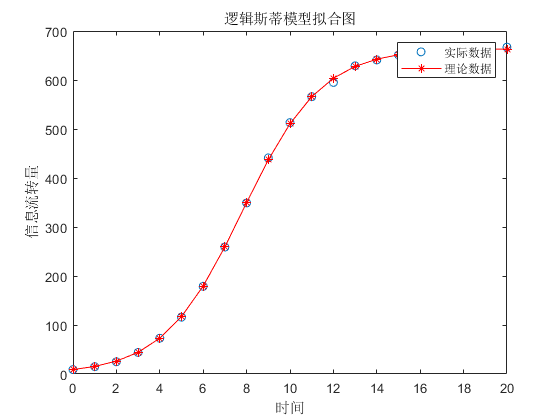
\includegraphics[scale=1]{逻辑斯蒂模型拟合图.png}
	\caption{逻辑斯蒂模型拟合图}
\end{figure}\par
我们将第0天作为$t=0$,将第20天作为$t=20$,对模型的解进行拟合优度检验,得到:
$$
SSR=\sum_{i=0}^{100}{\left( \hat{y}_i-\bar{y} \right) ^2},SST=\sum_{i=0}^{100}{\left( y_i-\bar{y} \right) ^2}
$$
$$
R^2=\frac{SSR}{SST}
$$\par
再利用MATLAB对以上算式进行求解,可以得出:
$$
SSE:120.9
$$
$$
R^2:0.9999
$$\par
即可看出所得结果与原数据相比的可决系数为0.9999,那么本文所展现的模型的匹配程度接近于为$100\%$,那么可以认为这个模型展现了网络信息真实的传播情况。
\subsection{问题二的模型建立与求解}
设初始人口$x_0$<$x_m$,由方程(2)得$t\rightarrow \infty ,x\rightarrow x_m$,对(1)求导$x''=\left( 1-2x/x_m \right) $,经过分析可知信息传播速率的极值点是x=/$x_m$/2,即当x=/$x_m$/2时信息传播速率最大,前一半为快速增长期.后一半为慢速增长期。该模型曲线有三个显著特征:一是单调递增性;二是增长有限性;三是形状为S形。\par
将公式(2)变式为时间随信息流转量的公式(4)后将$x=/x_m/2$以及问题一的计算结果代入可以得到传播速度最快的时间点。\par
\begin{equation}
	t=-\frac{\ln \left( \frac{\frac{x_m}{x}-1}{\frac{x_m}{x_0}-1} \right)}{r},
\end{equation}\par
计算得到\par
$$
t=7.80809h
$$\par
之后使用遍历的方法对其进行检验,设置初始时间为5h,步长为0.01,对公式(3)中的每一个点进行斜率求解并得到每一个时间点的信息传播速率如图3。
\begin{figure}[h]
	\centering
	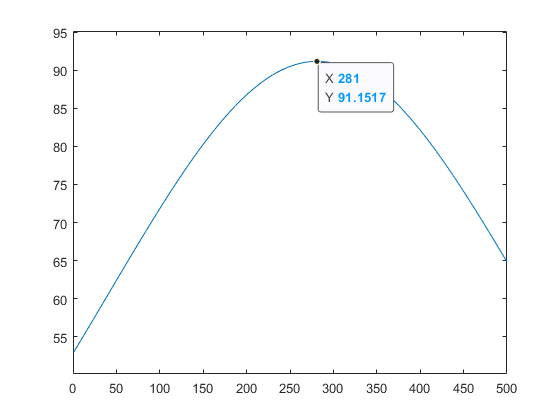
\includegraphics[scale=0.9]{信息传播速率.png}
	\caption{信息传播速率}
\end{figure}\par
检验得到在步长为0.01时,在时间为$t=5+0.01*281=7.81h$时达到最大的传播速率为91.1517,与上述的结果一致,因此可以得到传播速度最快的时间点\par
$$
t=7.809h
$$\par
\subsection{问题三和问题四的模型求解}
针对问题三,直接将模型进行推广,在公式(3)中代入$t=28h$得到28h时的信息流转量\par
$$
x(28)=663.998438
$$\par
针对问题四,在公式(3)中可以得到最终的信息流转量即为最大的的信息流转量\par
$$
x_m=664.0086
$$
\subsection{问题五的模型求解}
通过分析可以得到在传播环境不变时信息的传播速度仅和当前的信息流转量有关,因此控制信息传播的范围十分关键。\par
在前面问题的求解中可以发现,在本文的假设中,信息传播速度最快是在信息流转量量达到$x_m/2$的时候,因此可以知道,如果想要达到最快速的传播效果,使得流转量保持在最大流转量的一半是个最好的办法。同理,为了控制传播速度,需要尽可能在传播开始时加以限制。\par
信息传播速度的快慢对于信息传输的质量和效果都有着非常重要的影响,因此保持适当的传播速度是非常关键的。以下是一些控制信息传播速度的方式,以及它们的有效性:\par
提供更全面的信息: 通过提供更全面的信息,可以让接收者在接收到信息之前对信息有更好的理解,从而减少误解和恶意解读。这种方式可以缓慢传输速度,并大大降低误解和讽刺的风险。\par
限制信息来源:限制大量的信息来源将有助于减少失实和产生错误信息的可能性。通过提供对信息源的认证,可以降低不正确或有害信息的传播速度和影响。\par
传播媒介限制:传播媒介的限制对信息传输速度也有着重要的影响。限制信息的传播媒介可能包括禁止某些媒介的使用或向接收者暂缓信息的提供。\par
实施防火墙:防护墙可以限制未经批准的访问和活动,从而限制信息的传播。这对于网络和集成系统中实施访问控制非常有效。\par
以上控制传播速度的方式是有效的,但是需要考虑社会和政治因素。比如,在禁止信息的传播过程中,可能会存在严重的审查制度和恶意利用的可能性,可能会导致有价值和真实性的信息被删除或掩盖。因此,限制信息的传播必须在平衡公共需求和个人自由权利之间进行权衡。\par
	%Reference
\begin{thebibliography}{40}
	\bibitem{ref1}司守奎,孙玺菁.数学建模算法与应用[M].国防工业出版社,2011(8):270-275
	
	
	
	
\end{thebibliography}
\newpage
\newgeometry{left=1.50cm,right=0.5cm,top=3.00cm,bottom=3.0cm}	%修改附录代码的几何页面

\begin{center}
	\sihao \heiti 附录1
	
	
	\fontsize{10pt}{16pt}		\selectfont	
		\begin{lstlisting}[ language=MATLAB,numbers=left,numberstyle=\tiny,keywordstyle=\color{blue!70},commentstyle=\color{red!50!green!50!blue!50},frame=shadowbox, rulesepcolor=\color{red!20!green!20!blue!20},escapeinside=``,xleftmargin=2em,xrightmargin=2em,aboveskip=1em] 
		%population.m函数文件
		function g = population(x,t)
		g = x(1)./(1+(x(1)/9-1)*exp(-x(2)*t));  
		end		
	\end{lstlisting}
	\begin{lstlisting}[ language=MATLAB,numbers=left,numberstyle=\tiny,keywordstyle=\color{blue!70},commentstyle=\color{red!50!green!50!blue!50},frame=shadowbox, rulesepcolor=\color{red!20!green!20!blue!20},escapeinside=``,xleftmargin=2em,xrightmargin=2em,aboveskip=1em] 
		%问题一的求解
		clear;clc
		t = [0 1 2 3 4 5 6 7 8 9 10 11 12 13 14 15 16 17 18 19 20];
		p = [9.0 15.0 25.0 44.0	73.0 116.0 179.0 259.0 349.0 441.0 513.0 566.0 595.0 629.0 641.0 651.0 656.0 660.0 662.0 664.0 667.0];
		x0 = [200,3]; 
		x = lsqcurvefit('population',x0,t,p);
		p1 = population(x,t);
		plot(t,p,'o',t,p1,'-r*')
		title('逻辑斯蒂模型拟合图')
		xlabel('时间');
		ylabel('信息流转量');
		legend('实际数据','理论数据')l
	\end{lstlisting}
	\begin{lstlisting}[ language=MATLAB,numbers=left,numberstyle=\tiny,keywordstyle=\color{blue!70},commentstyle=\color{red!50!green!50!blue!50},frame=shadowbox, rulesepcolor=\color{red!20!green!20!blue!20},escapeinside=``,xleftmargin=2em,xrightmargin=2em,aboveskip=1em] 
	%问题二的验证
	clear;clc
	x=5:0.01:10;
	y=664.0086./(1+72.7787*exp(-0.5491*x));
	for i=1:length(x)-0.01
	k(i)=(y(i+1)-y(i))/(x(i+1)-x(i));
	end
	figure;plot(k)
	\end{lstlisting}	
	\begin{lstlisting}[ language=MATLAB,numbers=left,numberstyle=\tiny,keywordstyle=\color{blue!70},commentstyle=\color{red!50!green!50!blue!50},frame=shadowbox, rulesepcolor=\color{red!20!green!20!blue!20},escapeinside=``,xleftmargin=2em,xrightmargin=2em,aboveskip=1em]
	%求解数据
时间	 信息流转量
0   	9.000004066
1   	15.43220364
2   	26.27700362
3   	44.22321737
4    	73.02260105
5   	117.0354023
6    	179.5178976
7    	259.5305055
8   	349.4808848
9   	436.9299826
10   	510.7291483
11	    565.9279497
12   	603.5998035
13   	627.7298137
14	    642.5636496
15	    651.4534705
16   	656.7000081
17	    659.7683926
18	    661.5533858
19	    662.5885706
20  	663.187835

28	    663.998438
\end{lstlisting}
\end{center}
\end{document}